\section{Background}

Optimization is the act of finding the minimum or maximum of a function, called the objective function \cite{groetschel1995}. In combinatorial optimization, the domain of this function is typically finite\cite{groetschel1995}. Although selecting the best solution from finite possibilities may seem trivial, these functions can become extremely complex at even moderate size. When problems become too difficult to find the optimal solution, algorithms can be designed to find approximate solutions \cite{groetschel1995}. 

A special case is Quadratic Unconstrained Binary Optimization (QUBO). The goal is to maximize/minimize a quadratic function that takes either 0 or 1 as a variable without other constraints on the variable \cite{punnen2022}. The difference between maximization and minimization is simply a flip of the sign of the cost function. This problem can be written as follows:
    \begin{equation} 
        \text{min/maximize: } C(x) =\quad x^T Q x + c^T x \\
        \end{equation}
        \centerline{$x \in \{0,1\}^n, Q \in \mathbb{R}^{n \times n}, c \in \mathbb{R}^n$ }
        \vspace{+1mm}

QUBO problems are NP-complete, meaning they are an NP problem (nondeterministic polynomial time) and NP-hard. A problem is said to be NP-hard if an algorithm to solve it can be translated into solving any other NP problem \cite{wolfram}. QUBO can be applied to problems such as MaxCut, traveling salesman, and scheduling \cite{punnen2022}. Since they are NP-hard, it is very difficult for a classical algorithm to find the exact or approximate solution. People are looking to leverage quantum techniques such as QAOA to help solve these types of problems.
    
\subsection{MaxCut}
MaxCut is a type of problem that can always be formulated as a QUBO and is one of the most difficult combinatorial optimization problems to solve \cite{CommanderMaxCut}. MaxCut involves a graph with vertices (or nodes) V connected by edges E (that may be weighted). The goal is to find the partition of vertices with the highest weight. The weight of a "cut" is the sum of the weights of the edges that connect the vertices from different sets. 
\begin{figure}[H]
    \centering
    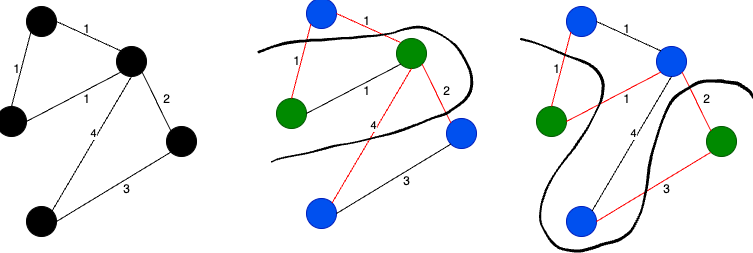
\includegraphics[width=1\linewidth]{images/MaCutExample.drawio.png}
    \caption{a) Example of a graph for MaxCut. b) Example cut with weight = 1 + 1 + 2 + 4 = 8. c) A different cut with weight = 1 + 1 + 2 + 3 = 7.}
    \label{fig:2.1}
\end{figure}

\subsubsection{Formulation}
Consider an undirected graph G = (V, E), where V is the set of vertices, E is the set of edges, and $w_{ij}$ is the weight of the edge that connects vertex i and j. A cut is the division of vertices into two subsets (0 and 1). The weight of the cut is the sum of the edges that connect vertices of different sets. This weight is represented by the cost function:

    \begin{equation} 
        C(x) = \sum_{i,j=1}^{n} W_{ij} x_i(1-x_j)
    \end{equation}

\begin{figure*}[ht]
    \centering
    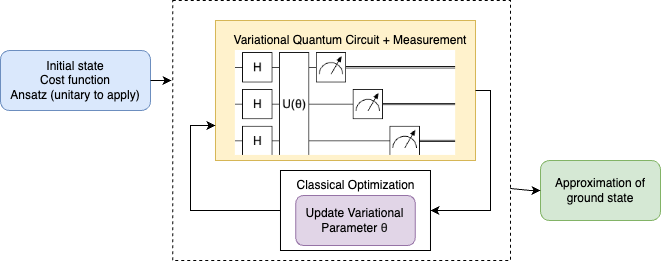
\includegraphics[width=0.8\linewidth]{images/VariationalDiagram.drawio.png}
    \caption{Diagram of variational quantum algorithms}
    \label{fig:enter-label}
\end{figure*}

\subsubsection{MaxCut to QUBO}
As explained before, MaxCut can be formulated as a QUBO. Here we reformulate the MaxCut cost function in accordance with QUBO:
\vspace{-2mm}
\begin{equation} 
        Q_{ij} = -W_{ij} \hspace{1.5cm} c_i = \sum_{j=1}^{n} W_{ij} 
    \end{equation}
\vspace{-2mm}
    \begin{equation} 
        C(x) = \sum_{i,j=1}^{n} x_i Q_{ij} x_j + \sum_{i=1}^{n} c_i x_i = x^T Q x + c^T x 
    \end{equation}

\subsubsection{Classical Solutions}
Since this is an NP-hard problem, an approximation algorithm is the best solution. First, we should define the approximation ratio:

\begin{equation} 
        \alpha = \frac{C}{C_{max}}
    \end{equation}

where C is the cost associated with the solution output and $C_{max}$ is the cost associated with the optimal solution. It is known that achieving an approximation ratio higher than 16/17 $\approx$ 0.941 is an NP-hard problem \cite{hastad2001}. The best classical approximation algorithm is the Goemans-Williamson algorithm, which guarantees an approximation ratio of $\alpha \geq 0.878$ using semidefinite programming techniques \cite{GWalgorithm}. Other solutions for more specific graphs use techniques such as greedy randomized search, variable neighborhood search, and path-relinking algorithms \cite{GWalgorithm}. Therefore, leveraging quantum techniques to solve optimization problems such as MaxCut is a highly researched topic.

\subsection{Variational Quantum Algorithms}
Variational Quantum Algorithms are a broader category of quantum algorithms that include QAOA. These algorithms aim to find the ground state of a Hamiltonian (H) using the variational principle \cite{vqa2021}. The variational principle states that the ground state energy is always less than or equal to the expectation value of H calculated with the trial wave function \cite{vqa2021}.

\begin{equation} 
        E_0  \leq  \braket{\psi|H|\psi}
    \end{equation}

So, by varying $\ket{\psi}$ until the expectation value is minimized, we can obtain an approximation for the ground state and its energy. A diagram of how these algorithms work is shown in Fig. 2. 

The first step is to encode the problem into a cost function that we can optimize \cite{vqa2021}. We have already defined our cost functions for MaxCut, in equations (2) and (4). The minimum of the cost function should correspond to the solution of the problem \cite{vqa2021}. The next step is to develop an ansatz, a quantum circuit that will map the input state to the desired ground state. There are many different possible ansatzes depending on the problem. For QAOA, we have a "quantum alternating operator ansatz", which sequentially applies alternating unitaries, $U_M$ and $U_C$, to get to the ground state \cite{vqa2021}. $U_M = e^{-i \beta H_M}$ and $U_C = e^{-i \gamma H_C}$ where the parameterized values are $\theta = (\gamma, \beta)$ \cite{vqa2021}.

This information is then given to a quantum computer to efficiently find the output of the cost function. This result is given to a classical computer to optimize the parameters. Many methods exist for this optimization, including stochastic gradient descent \cite{vqa2021}. Once the parameters are optimized, they are given back to the variational quantum circuit to perform another measurement. This hybrid quantum-classical loop can be repeated many times to reach the desired result.

\subsubsection{Variational Quantum Eigensolver}
The variational quantum eigensolver was first introduced by Peruzzo et al. \cite{vqe2014} and later improved upon by McClean et al. \cite{vqeExt2016}. The objective is to solve for the lowest energy state of a given Hamiltonian by using the variational quantum algorithm techniques described in the previous section. The cost function is defined as:

\begin{equation} 
        E_{VQE} =  min_\theta \braket{0|U^\dagger (\theta)\hat{H} U(\theta)|0}
    \end{equation}

where the initial state is typically $\ket{0}$ and the ansatz is the parameterized unitary U($\theta$). The state is then iteratively optimized by varying the parameters $\theta$ towards the optimal parameters \cite{vqeReview}.

This algorithm was proposed as an alternative to phase estimation that reduces the requirements for coherent evolution \cite{vqe2014}. Quantum phase estimation does offer an exponential speedup over classical methods, but it requires many quantum operations and thus needs long coherence times and minimal noise \cite{vqe2014}. VQEs take advantage of the combination of classical and quantum resources while still providing an exponential speedup over classical algorithms, making it a more useful near-term algorithm than phase estimation. 

\subsubsection{Quantum Adiabatic Algorithm}
The Quantum Adiabatic Algorithm was proposed in 2001 by Fahri et al. \cite{qaa2001}, which takes advantage of the adiabatic theorem. We know that quantum systems evolve in time according to the Schrodinger equation:

\begin{equation} 
        i \frac{d}{dt} \ket{\psi(t)} = H(t) \ket{\psi(t)}
    \end{equation}

where $\ket{\psi(t)}$ is the wave function and H(t) is the time-dependent Hamiltonian. The adiabatic theorem states that if we start in the ground state of a time-dependent Hamiltonian and slowly evolve H, the resulting state $\ket{\psi(t)}$ will be the ground state of the final Hamiltonian \cite{qaa2001}.

We can start by choosing a Hamiltonian $H_S$ with a simple and known ground state. For any problem $H_P$ with a complex ground state, we can find this state by slowly evolving $H_S$ to $H_P$ \cite{qaa2001}. We define H(t) over a time period $0 \leq t \leq T$, where H(0) = $H_S$ and H(T) = $H_P$ \cite{qaa2001}. This relates to QAOA because as the number of layers in QAOA increases towards $\infty$, the algorithm will find the optimal solution according to the adiabatic theorem \cite{farhiQAOA}.

\subsubsection{Trotterization}
If we have a Hamiltonian $H_C = H_1 + H_2$, then we can write the time evolution as follows:

\begin{equation} 
        U(t) = e^{-i H t /\hbar} = e^{-i (H_1 + H_2)t/\hbar}
    \end{equation}

For matrices that commute, we know that $e^{A+B} = e^A e^B$. However, this does not apply to matrices that do not commute. Instead, there exists an approximation called the Trotter Product Formula, which finds that:

\begin{equation} 
        e^{-i (A + B) t} \approx (e^{-iAt/r}e^{-iBt/r})^r
    \end{equation}

where r is known as the Trotterization depth \cite{trot2023}. The higher r is, the more accurate the approximation will be.